\documentclass[draft,grl]{agujournal2018}
%\documentclass[]{agujournal2018}
\usepackage{apacite}
\usepackage{natbib}


\usepackage{url}
\usepackage{lineno}
\usepackage{trackchanges}
\soulregister\citet7
\soulregister\citep7
\soulregister\ref7
\addeditor{JKP} 


%\draftfalse
\journalname{Geophysical Research Letters}

%custom packages
\usepackage{amsmath,amssymb,amsfonts,amsthm}
\usepackage{comment}
\usepackage{booktabs}
% custom commands
\newcommand\be{\begin{equation}}
\newcommand\ee{\end{equation}} 
\newcommand\bra{\langle}
\newcommand\ket{\rangle}
\newcommand\om{\omega}
\newcommand\tom{\tilde{\omega}}
\newcommand\tg{\tilde{g}}
\newcommand\tp{\tilde{p}}
\newcommand\tG{\tilde{G}}
\newcommand\El{\mathcal{L}}
%\usepackage{layouts}
%\printinunitsof{in}\prntlen{\textwidth} % check scales in the document
\linenumbers

% THIS IS THE LINENO PATCH TO WORK WITH AMSMATH
\newcommand*\patchAmsMathEnvironmentForLineno[1]{%
	\expandafter\let\csname old#1\expandafter\endcsname\csname #1\endcsname
	\expandafter\let\csname oldend#1\expandafter\endcsname\csname end#1\endcsname
	\renewenvironment{#1}%
	{\linenomath\csname old#1\endcsname}%
	{\csname oldend#1\endcsname\endlinenomath}}% 
\newcommand*\patchBothAmsMathEnvironmentsForLineno[1]{%
	\patchAmsMathEnvironmentForLineno{#1}%
	\patchAmsMathEnvironmentForLineno{#1*}}%
\AtBeginDocument{%
	\patchBothAmsMathEnvironmentsForLineno{equation}%
	\patchBothAmsMathEnvironmentsForLineno{align}%
	\patchBothAmsMathEnvironmentsForLineno{flalign}%
	\patchBothAmsMathEnvironmentsForLineno{alignat}%
	\patchBothAmsMathEnvironmentsForLineno{gather}%
	\patchBothAmsMathEnvironmentsForLineno{multline}%
}
% the patch comes from http://phaseportrait.blogspot.com/2007/08/lineno-and-amsmath-compatibility.html

\begin{document}



\title{Back to Einstein: \change{how to include}{including} burial in fluvial sediment diffusion models\remove{?}}

\authors{James K. Pierce \affil{1}and Marwan A. Hassan\affil{1}}
\affiliation{1}{Department of Geography \\University of British Columbia}
\correspondingauthor{James Kevin Pierce}{kpierce@alumni.ubc.ca}

\begin{keypoints}
\item \change{We develop a random walk model of objects in intermittent transport through an environment with traps}{We develop a random walk model of bedload tracers diffusing through a river as they gradually become buried}
\item \change{Its solution provides three ranges of diffusion, two of which are anomalous}{The model predicts three diffusion ranges as the observation time increases, one normal and two anomalous}
\item \change{We apply the model to sediment transport in rivers to clarify the scale dependence of bedload diffusion}{We relate these ranges to sediment motion, rest, and burial timescales and clarify their generating processes}

\end{keypoints}

\begin{abstract}
Sediment grains transport through gravel bed rivers in cycles of motion and rest.
When grains rest on the surface, material transported from upstream can bury them.
The surface shields buried grains from the flow, so they can be immobile for long time periods.
These immobile periods can dominate sediment diffusion characteristics.
Although investigators have recognized the impact of sediment burial on diffusion, existing models do not usually incorporate it.
In this study, we present the first random walk model incorporating sediment burial and the duration of individual sediment motions and solve it analytically.
The model predicts three sediment diffusion ranges with distinct scaling characteristics in each.
We relate the crossover times dividing these ranges to measurable transport parameters and describe each range from underlying physical processes.
\add{This work has implications for all researchers concerned with coarse material moving in river channels on grain to geomorphic scales.}
\remove{
Our developments provide new geophysical perspective on the anomalous scaling of fluvial sediment transport.}
\note{Who is the audience?}
\end{abstract}

\section{Introduction}

\add{A group of bedload tracers added to a river channel spreads apart through time due to differences in the downstream transport characteristics and conditions encountered by one grain and the next in a process called bedload diffusion.}
Many environmental problems including contaminant transport \citep[e.g.,][]{Macklin2006}, channel stability \citep[e.g.,][]{Hassan2017}, and aquatic habitat restoration \citep[e.g.,][]{Gaeuman2017} rely on our ability to predict this diffusion, so the topic has been researched intensively for over 80 years.
Diffusion is usually quantified by the time dependence of the positional variance of the group of tracers.
With the scaling $\sigma_x^2 \propto t$, the diffusion is said to be normal, since this is found in the classic problems \citep[e.g.,][]{Einstein1905,Taylor1920}.
However, with the scaling $\sigma_x^2 \propto t^\gamma$ with $\gamma \neq 1$, the diffusion is said to be anomalous \citep{Sokolov2012}. 
If $\gamma>1$, it is said to be super-diffusive; while if $\gamma <1$, it is said to be sub-diffusive \citep{Metzler2000}.
Hans Albert Einstein developed the first model of bedload diffusion to describe his comprehensive \add{flume} experiments visually tracking painted grains \remove{in a flume} \citep{Ettema2004,Einstein1937}.
\add{Interpreting individual bedload trajectories as a sequence of random steps and rests, }Einstein originally concluded \change{that bedload transport shows}{that a group of bedload tracers undergoes} normal diffusion.

\change{After Einstein}{More recently}, Nikora and coworkers \add{(hereafter ``Nikora'')} \change{recognized}{realized} coarse sediment \add{tracers} \remove{moving through river channels} can show either anomalous or normal diffusion depending on the \change{timescale of observation}{length of time they have been tracked} \citep{Nikora2001a,Nikora2002}.
\add{From numerical simulations and experimental data, Nikora discerned three scaling ranges $\sigma_x^2 \propto t^\gamma$ as the observation time increased.
They associated the first range with ``local'' timescales being less than the interval between subsequent collisions of moving grains with the bed, the second with ``intermediate'' timescales being less than the interval between successive resting periods of grains, and the third with ``global'' timescales composed of many intermediate timescales.
Nikora proposed super-diffusion in the local range, anomalous or normal diffusion in the intermediate range, and sub-diffusion in the global range. Although Nikora described local range super-diffusion as a consequence of the smoothness of bedload trajectories between subsequent collisions of moving grains with the bed, they did not completely pin down the physical mechanisms generating intermediate and global range diffusion.
In this paper, we refer to diffusion having multiple scaling ranges as being ``scale dependent'', and we set out to better understand the physical processes giving rise to local, intermediate, and global bedload diffusion ranges.}
\remove{
This is a significant issue since it implies diffusion models should be scale dependent, and it renders experimental data contingent on their observation timescales.
Nikora et al. identified three ranges of diffusion from Newtonian simulations and experimental data and termed these ranges local, intermediate, and global in order of increasing timescale.
They determined that $\sigma_x^2$ scales with a different power of time in each range, and they concluded this scaling could be anomalous or normal.}

\change{Recent studies}{Experiments} support \change{the Nikora et al.}{Nikora's conclusion} \change{that bedload diffusion shows multiple scaling ranges}{of multiple bedload diffusion scaling ranges}, but they do not \change{show}{ provide} consensus on the expected number of ranges or their scaling properties.
\add{This lack of consensus likely results from resolution issues.
For example, measurements have been conducted at high temporal resolution for short periods, sampling local and intermediate ranges} \citep[e.g.,][]{Furbish2012}; \add{moderate temporal resolution for moderate periods, sampling only the intermediate range} \citep[e.g.,][]{Einstein1937,Yano1969,Nakagawa1976}; \add{moderate temporal resolution for long periods, sampling the intermediate and global ranges} \citep[e.g.,][]{Martin2012}; \add{or at low temporal resolution for long periods, sampling only the global range} \citep[e.g.,][]{Bradley2010,Phillips2013,Bradley2017}.
\add{As a result, three ranges can be identified by patching together multiple datasets} \citep[e.g.,][]{Zhang2012}\add{, but they are not resolved by any one dataset.}

\add{
Modelling studies display similarly patchy understanding.
Using Newtonian simulations, \citet{Nikora2001a} resolved local and intermediate ranges, while \citet{Bialik2012} resolved all three ranges.
However, direct computations are impractical at field scales and provide limited physical insight, motivating alternative approaches.
One option is to generalize the random walk model of Einstein.
Einstein's model treats bedload trajectories as instantaneous steps interrupted by durations of rest which lie on statistical distributions \citep{Hassan1991}.
This derives only one range of normal diffusion }\citep[e.g.,][]{Einstein1937,Hubbell1964,Nakagawa1976}.
\add{
More recently, researchers generalized Einstein's model in a few different ways to include the interval of motion.  
\citet{Lisle1998} assumed particles moved for random intervals with a deterministic velocity, while \citet{Fan2016} described motions with random intervals and velocities dictated by an underlying Langevin equation.
\citet{Lajeunesse2018} took an alternate perspective developing identical governing equations as \citet{Lisle1998}.
By including the motion interval, these approaches provide two ranges of diffusion -- a local range super-diffusion and an intermediate range normal diffusion, but they do not provide a global range.
To model the global range, \citet{Wu2019} took a different path from Einstein. They retained the instantaneous motion assumption but included the possibility that sediment becomes buried as it rests on the bed.
By including burial, this approach also provides two ranges of diffusion -- an intermediate range normal diffusion and a global range super-diffusion, but it does not provide a local range.
Therefore, although no Einstein-type model of three ranges has been developed, these earlier works suggest the required components are (1) non-zero motion intervals and (2) sediment burial.}

In this study, we develop the first model of bedload diffusion describing local, intermediate, and global \change{ranges of diffusion}{diffusion ranges} by \add{incorporating these two components into Einstein's original model.}\remove{the original diffusion model of \citet{Einstein1937}}
Einstein was a giant in river geophysics and fostered an entire paradigm of research leveraging and generalizing his stochastic methods \citep[e.g.,][]{Hubbell1964, Yano1969, Yang1971, Gordon1972, Nakagawa1976}.
Einstein's model can be viewed as a special case of the continuous time random walk (CTRW) developed by \citet{Montroll1965} in condensed matter physics to describe the diffusion of charge carriers in solids.
\remove{Our generalization of Einstein's model has two components.
First, we include the duration and velocity of motions in place of instantaneous steps, and second, we add in the sediment burial process.}
To \change{develop this generalization}{incorporate motion intervals and sediment burial}, we leverage the multi state CTRW developed by \citet{Weiss1976, Weiss1994} that extends the CTRW of \citet{Montroll1965}.
Below, we develop the model in section \ref{sec:model} and solve it in section \ref{sec:solution}. Finally, we discuss the predictions of our model and its implications for \change{scale dependent bedload transport}{local, intermediate, and global ranges of bedload diffusion} in sections \ref{sec:discussion} and \ref{sec:conclusion}.

\section{Bedload diffusion with burial as a multi state random walk}
\label{sec:model}

Following Einstein, we describe bedload transport as a random walk between mobile and immobile states.
However, in contrast to Einstein, we carefully distinguish two states of immobility: grains can be immobile on the surface, which we refer to as the ``resting state'', or grains can be immobile within the sub-surface, which we refer to as the ``burial state''.
To model bedload transport with both of these immobile states, we construct a three-state random walk where the states are motion, rest, and burial, and we label these states as $i=2$ (motion), $i=1$ (rest), and $i=0$ (burial).
Our development of the governing equations for the three state walk follows \citet{Weiss1994}, and our incorporation of the sediment burial process is similar to \citet{Schmidt2007}.
In our model, times spent moving or resting on the bed surface are random variables characterized by \change{exponential}{probability} distributions, and moving grains have a constant velocity $v$.
Within the model, we consider burial to be a relatively long lasting condition that has some probability to occur when grains resting on the surface are covered by transported sediment.
The probability of burial per unit time (burial rate) is considered constant, so the probability that grains become buried increases with the time they rest.

% describe meaning of sojourns and g_i/G_i/theta_i
Our derivation hinges on the concept of a sojourn in the state $i$ \citep{Weiss1994}.
When a grain enters a state $i$ at some time $t_0$ and position $x_0$, then leaves \change{a}{the} state at some other time $t_1$ and position $x_1$, we say that the grain has completed a sojourn in the state $i$. \add{We denote }the joint probability density for a complete sojourn in the state $i$ of time $t = t_1-t_0$ and displacement $x = x_1-x_0$ \remove{is denoted}{as} $g_i(x,t).$ 
Similarly, we consider incomplete sojourns. If a grain begins a sojourn in the state $i$ at $(t_0,x_0)$ and the sojourn is still ongoing at $(x_1,t_1)$, the joint probability density to find the grain is $G_i(x,t)$.
We refer to $g_i$ and $G_i$ as the complete and incomplete propagators, since they move probability through space-time and are associated respectively with complete and incomplete sojourns.

Our target is the probability distribution $p(x,t)$ to find a grain at $x,t$ if we know it started at $(x,t)=(0,0)$; that is, if it started with the initial distribution $p(x,0)=\delta(x)$.
We denote the initial probabilities to be at rest or in motion as $\theta_1$ and $\theta_2$. Normalization requires $\theta_1+\theta_2=1$.
Our derivation has two main stages.
First, we introduce and solve for a set of joint probabilities \change{associated with}{describing} transitions of a grain from one state to another.
Second, we use these quantities to solve for the probabilities that a grain is in state $i$ having position $x$ at time $t$.
Afterward, we sum these latter distributions over all states $i$ to derive the joint distribution that a grain is in any state at $(x,t)$.

% derive omegas
Now we begin the first stage of the derivation.
Grains at rest may be trapped by burial.
For simplicity, we model burial as long lasting enough to be effectively permanent \citep[e.g.,][]{Wu2019}, and we assume grains resting on the surface can be buried with constant rate $\kappa$.
Equivalently, we could say the mean time required for a resting grain to become buried is $1/\kappa$.
From this assumption, the probability that a grain is not trapped after a time $t$ at rest obeys a survival function: $\Phi_F(t) = e^{-\kappa t}$ ($F$ is for ``free''). Likewise, the probability that it is trapped after resting for a time $t$ is the complement: $\Phi_T(t) = 1-\Phi_F(t)$ ($T$ is for ``trapped'').
We introduce $\omega_{1T}(x,t)$, $\omega_{1F}(x,t)$, and $\omega_2(x,t)$ as the joint probabilities to find a grain at $(x,t)$ having just completed a sojourn.
The subscript ${1T}$ denotes the completion of a rest sojourn due to trapping by burial, while $1F$ denotes the completion of a rest sojourn due to motion.
Similarly, the subscript $2$ denotes the completion of a motion sojourn due to resting.
We link the $\omega$'s in integral equations using an argument similar to \citet{Weiss1994}:
\begin{alignat}{2}
&\om_{1T}(x,t) &&= \theta_1\Phi_T(t)g_1(x,t) + \int_0^x dx' \int_0^t dt' \om_2(x',t')\Phi_T(t-t')g_1(x-x',t-t')\label{eq:x},\\
&\om_{1F}(x,t) &&= \theta_1\Phi_F(t)g_1(x,t) + \int_0^x dx' \int_0^t dt' \om_2(x',t') \Phi_F(t-t') g_1(x-x',t-t'),\label{eq:xy}\\
&\om_2(x,t) &&= \theta_2 g_2(x,t) + \int_0^x dx' \int_0^t dt' \om_{1F}(x',t')g_2(x-x',t-t'). \label{eq:y}
\end{alignat}
The first equation can be understood as follows: $\omega_{1T}(x,t)$ describes the probability \add{density} that a sojourn in the state $1$ ends due to trapping at $(x,t)$. This quantity has two contributions. The first contribution represents the possibility that the grain started at $(x,t)=(0,0)$ in the $i=1$ state (with probability $\theta_1$), propagated a distance $x$ and a time $t$ in the $i=1$ state (with probability density $g_1(x,t)$), was trapped (with probability $\Phi_T(t)$), and is now at $(x,t)$. 
The second contribution describes the possibility that the grain was in a motion sojourn which ended at $(x',t')$ when it came to rest. From here, it propagated from $(x',t')$ to $(x,t)$ at rest (with probability density $g_1(x-x',t-t')$) and was trapped during this sojourn (with probability $\Phi_T(t-t')$).
The reasoning is closely analogous for equations (\ref{eq:xy}) and (\ref{eq:y}).
Once the propagators are specified, we can solve (\ref{eq:x}-\ref{eq:y}) for the $\omega$'s to complete the first stage of the derivation.

% derive p's
The second stage of our derivation involves the joint probabilities of being in state regardless of whether a sojourn has just completed. We denote these by  $p_0(x,t)$ (trapped), $p_1(x,t)$ (rest), and $p_2(x,t)$ (motion), and we involve the $\omega$'s in their definition:
\begin{align}
p_0(x,t) &= \int_0^t dt' \omega_{1T}(x,t-t'), \label{eq:b}\\
p_1(x,t) &= \theta_1 G_1(x,t) + \int_0^x dx' \int_0^t dt' \omega_2(x',t')G_1(x-x',t-t'),\label{eq:a}\\
p_2(x,t) &= \theta_2 G_2(x,t) + \int_0^x dx' \int_0^t dt'  \omega_{1F}(x',t')G_2(x-x',t-t').\label{eq:z}
\end{align}
Equation (\ref{eq:b}) says that grains buried at any $(x,t)$ were trapped at $x$ from any earlier times.
The reasoning in (\ref{eq:a}-\ref{eq:z}) is the same as for (\ref{eq:x}-\ref{eq:y}) except we use the propagators for incomplete sojourns.
Equations (\ref{eq:b}-\ref{eq:z}) can be solved once the propagators are specified and the $\omega$'s are derived from (\ref{eq:x}-\ref{eq:y}).
Finally, we form the total probability density for a grain to be found at $(x,t)$ in any state.
This is simply 
\be p(x,t) = p_0(x,t) + p_1(x,t) + p_2(x,t). \label{eq:dist}\ee
This joint density was our target and is completely determined once (\ref{eq:x}-\ref{eq:z}) are solved.


\section{Specification of propagators and solution of model}
\label{sec:solution}
\add{
We assume sojourn times in the motion and surface rest states are exponentially distributed as this is suggested by experimental data }\citep[e.g.,][]{Yano1969,Einstein1937,Fathel2015, Martin2012}\add{, physical arguments }\citep[e.g.,][]{Furbish2016}\add{, and earlier modelling works} \citep[e.g.,][]{Fan2016,Wu2019}.
\add{We expect our conclusions will not be contingent on these assumptions, since all light tailed distributions are known to provide similar diffusion properties in random walks} \citep[e.g.,][]{Weiss1994,Weeks1998}.
\change{We consider sojourns in the rest state to occur for an exponentially distributed time interval given by the distribution}{We write the distribution of sojourn times in the rest state as}  $\psi_1(t) = k_1 e^{-k_1t}.$
The probability that a sojourn in this state lasts for at least a time $t$ is then $\Psi_1(t) = \int_t^\infty \psi_1(t)dt = e^{-k_1 t}$, and $1/k_1$ is the mean duration of a single rest.
Since grains do not move in the rest sojourn, the probability density that a grain is displaced by a distance $x$ in the rest sojourn in $\delta(x)$.
\change{Hence}{This means} the complete propagator for rest sojourns is $g_1(x,t) = \delta(x)\psi_1(t),$ or 
\be g_1(x,t) = \delta(x)k_1e^{-k_1t}.\label{eq:prop1} \ee
Likewise, the incomplete propagator for a rest sojourn is $G_1(x,t) = \delta(x)\Psi_1(t) = \delta(x)e^{-k_1t} = g_1(x,t)/k_1.$
The motion propagators are reasoned similarly. We consider motions to have a constant velocity $v$ and \change{exponentially distributed durations given by}{sojourn time distribution} $\psi_2(t) = k_2 e^{-k_2t},$
and $1/k_2$ is the mean duration of a single motion.
Since the velocity of motions is constant, the probability to find a grain at position $x$ in a motion sojourn is $\delta(x-vt)$, and the complete propagator for motion sojourns is 
\be g_2(x,t) = \delta(x-vt)k_2e^{-k_2t},\label{eq:prop2}\ee
while the incomplete propagator is $G_2(x,t) = g_2(x,t)/k_2$, as before.

Having defined the propagators  (\ref{eq:prop1}-\ref{eq:prop2}), we set out to solve (\ref{eq:x}-\ref{eq:z}) \change{and}{to} understand the diffusion expressed by the \change{trapping}{three state} model.
\note{Moved a major block to the supplementary information.}
\change{Using transform calculus, the joint distribution $p(x,t)$ is derived in appendix \ref{sec:appendixA}, and the moments $\bra x \ket$, $\bra x^2 \ket$, and ultimately the variance of position $\sigma_x^2(t)$ are derived in appendix \ref{sec:appendixB}.}{To keep the focus on the physics we have pushed the mathematical details into the supplementary information, where we derive the joint distribution $p(x,t)$, the moments $\bra x \ket$ and $\bra x^2 \ket$, and ultimately the variance of position $\sigma_x^2(t)$. }
With the shorthand notations $\xi = k_2 x/v$, $\tau = k_1(t-x/v)$, and $\Omega = (\kappa+k_1)/k_1$ \citep[cf.,][]{Lisle1998}, the joint distribution to find a grain at position $x$ at time $t$ \change{is}{comes out as} 
\begin{multline}
p(x,t) = \theta_1\mathcal{H}(\xi)\mathcal{H}(\tau)\Big[1-\frac{k_1}{\kappa+k_1}\Big(1-e^{-(\kappa+k_1)t}\Big)\Big]\delta(x) \\ + \frac{1}{v}e^{-\Omega \tau - \xi}\mathcal{H}(\xi)\mathcal{H}(\tau)\Big(\theta_1\Big[k_1\mathcal{I}_0\big(2\sqrt{\xi\tau}\big) + k_2\sqrt{\frac{\tau}{\xi}}\mathcal{I}_1\big(2\sqrt{\xi\tau}\big)\Big] \\ + \theta_2\Big[k_1\delta(\tau) + k_2 \mathcal{I}_0\big(2\sqrt{\xi\tau}\big)+k_1 \sqrt{\frac{\xi}{\tau}}\mathcal{I}_1\big(2\sqrt{\xi\tau}\big)\Big]\Big) \\
+ \frac{1}{v}\frac{\kappa k_2}{\kappa + k_1}e^{-\kappa \xi/(\kappa + k_1)}\mathcal{H}(\xi)\mathcal{H}(\tau)\Big[(\theta_1/\Omega)\mathcal{P}_2(\xi/\Omega,\Omega\tau) + \theta_2 \mathcal{P}_1(\xi/\Omega,\Omega\tau)\Big].
\label{eq:pdf}
\end{multline}
$\mathcal{H}$ is the Heaviside step function and we use the convention $\mathcal{H}(0)=1$.
The $\mathcal{I}_\nu$ are modified Bessel functions of the first kind, and the $\mathcal{P}_\mu$ are generalized Marcum Q-functions defined by $\mathcal{P}_\mu(x,y) = \int_0^y e^{-z-x}(z/x)^{(\mu-1)/2}\mathcal{I}_{\mu-1}(2\sqrt{xz})dz $ \citep{Temme1996}. Modified Bessel functions are common in one-dimensional diffusion problems \citep[e.g.,][]{Giddings1955, Daly2010}, and they have long been used to characterize the distribution of bedload tracers moving or resting on the surface \citep[e.g.,][]{Einstein1937,Hubbell1964, Bradley2012}. 
\begin{figure}[t]
	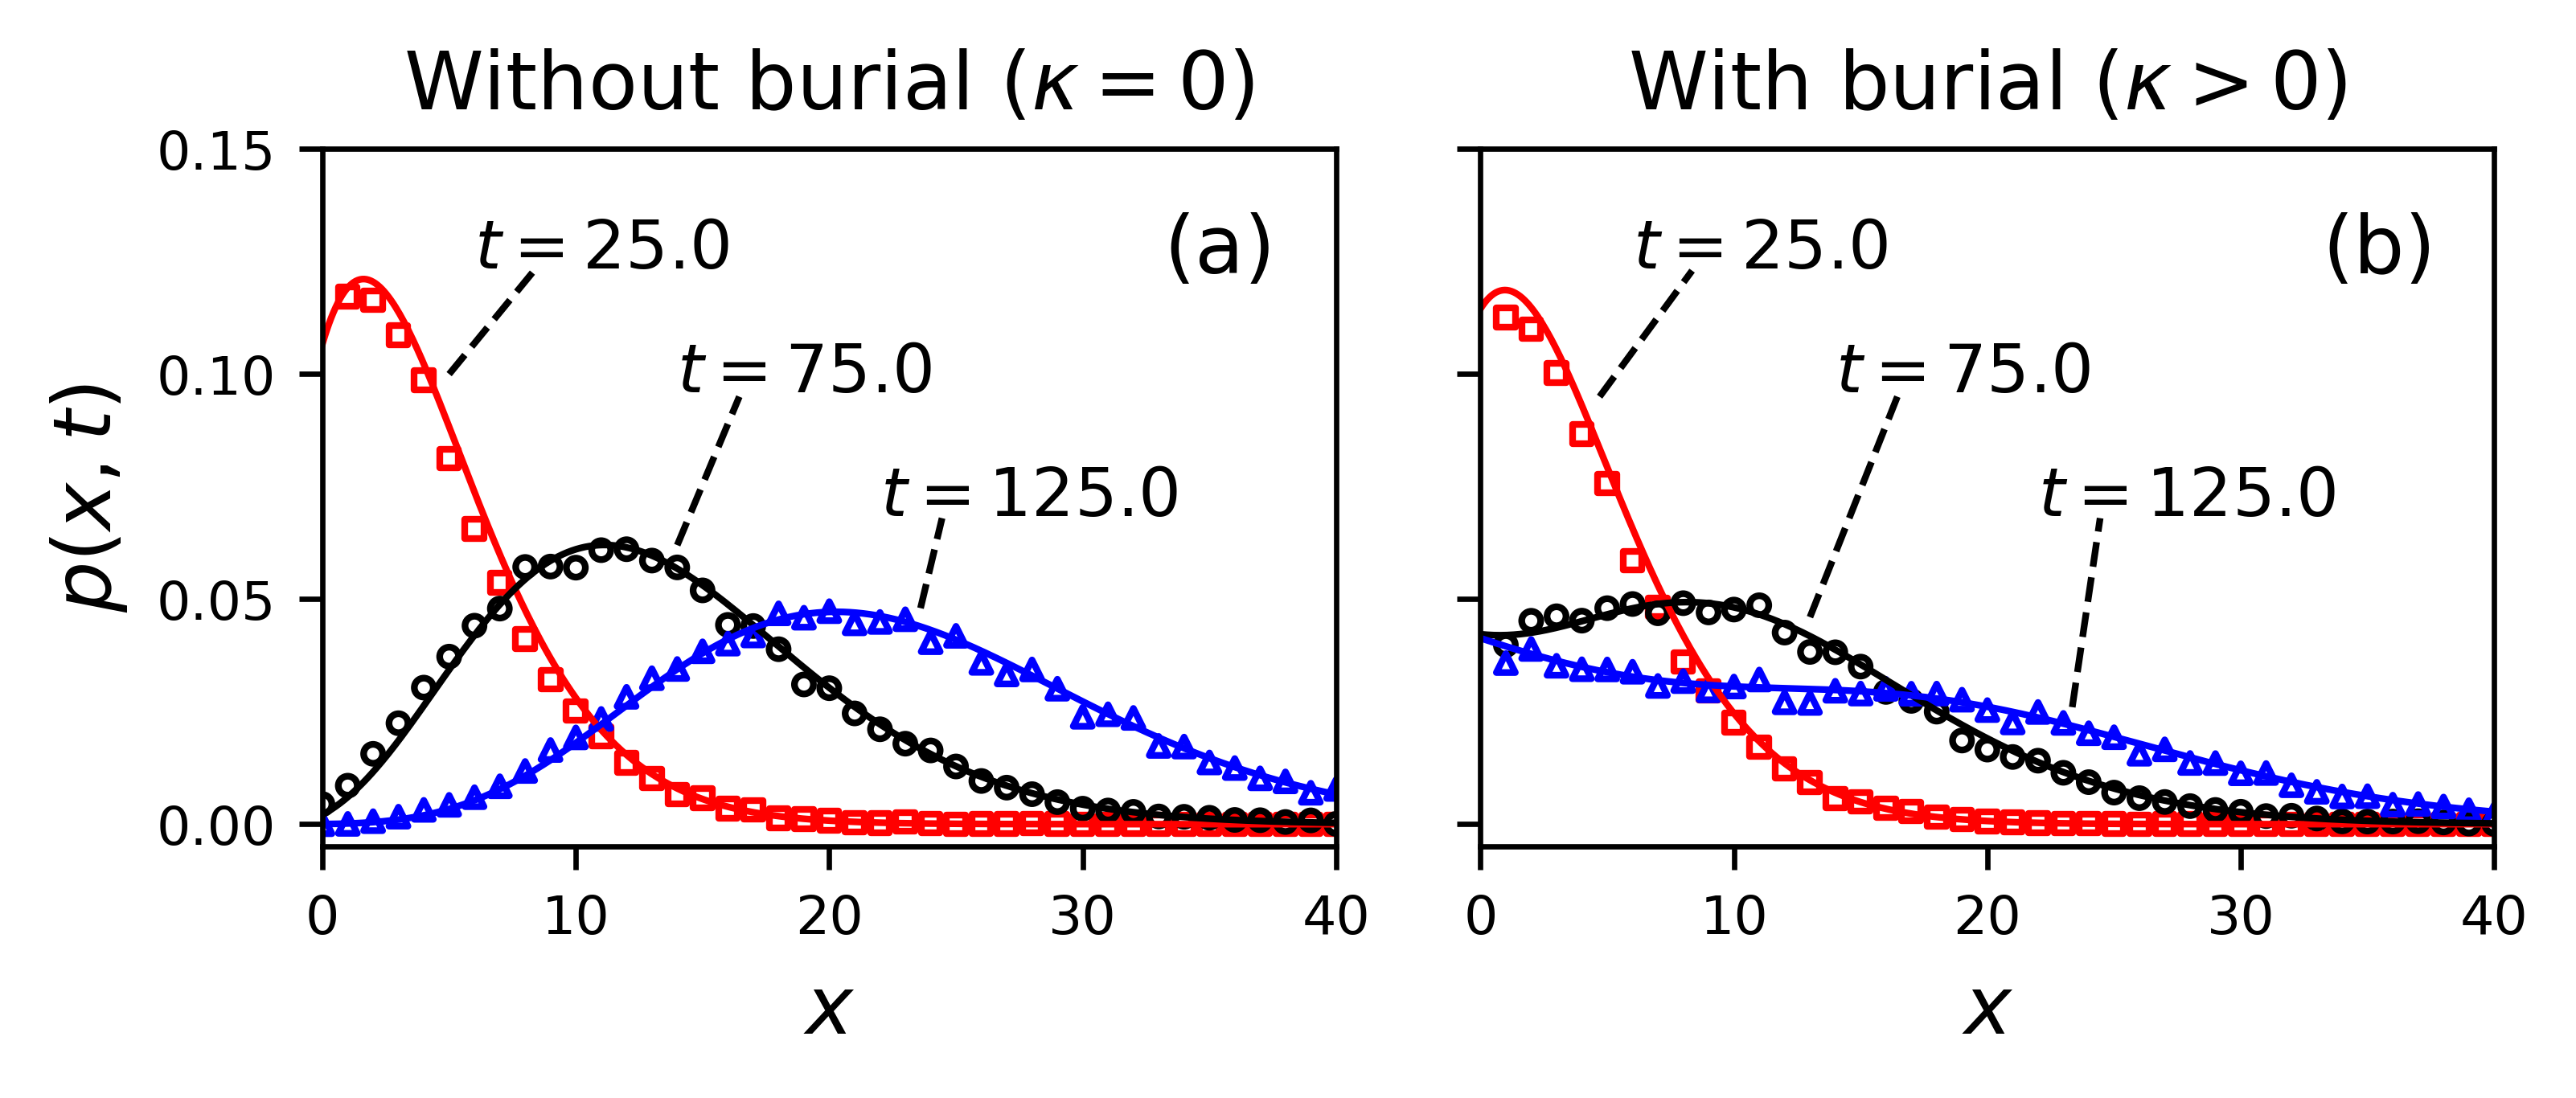
\includegraphics[width=\linewidth,keepaspectratio]{./figures/pdf-plot.png}
	\caption{Joint distributions for a grain to be at position $x$ at time $t$ are displayed for the choice $k_1=0.1$, $k_2=1.0$, $v=2.0$. Grains are considered initially at rest ($\theta_1=1$, $\theta_2=0$). The solid lines are the analytical distribution in equation (\ref{eq:pdf}), while the points are simulation results to show mathematical correctness. Colors pertain to different times. Units are unspecified, since our aim is to demonstrate the general characteristics of $p(x,t)$. Panel (a) shows the case $\kappa=0$ -- the absence of burial.
		In this case, the joint distribution tends toward Gaussian at large times \citep[e.g.,][]{Einstein1937,Lisle1998}. Panel (b) shows the case when grains have rate $\kappa = 0.01$ to become buried while resting.
		Because of burial, the joint distribution tends toward a more uniform distribution than Gaussian. This shows a redistribution of probability to smaller values of $x$ due to the burial process \citep[cf.,][]{Wu2019}. The redistribution is encoded mathematically by the Marcum Q-function terms in equation  (\ref{eq:pdf}). A similar tendency is seen in field studies of tracer dispersion in gravel bed rivers \citep[e.g.,][]{Hassan1994}.}
	\label{fig:pdfs}
\end{figure}

The Marcum Q-functions are \add{new to bedload transport and therefore merit some discussion. They are }convolutions between modified Bessel functions and decaying exponentials\change{. They }{and }were originally devised in relation to radar detection theory \citep{Marcum1960}. 
Conceptually, the Q-functions emerge in our context from the sediment burial process. According to our assumptions, resting grains can become buried in some interval of time with an exponential probability. Meanwhile, the probability that grains are resting \add{on the surface} follows a modified Bessel distribution \citep[e.g.,][]{Einstein1937,Lisle1998}.
As a result, the probability that sediment is resting and becomes buried involves the convolution structure of the Marcum Q-functions.
Consistent with this interpretation, terms involving these convolutions vanish when the burial rate is taken to zero $(\kappa \rightarrow 0)$.
Figure \ref{fig:pdfs} depicts the distribution (\ref{eq:pdf}) alongside simulations generated by a direct method based on evaluating the cumulative transition probabilities between states on a small timestep \citep[cf.,][]{Barik2006}\add{, illustrating the correctness of our derivations}. A link to the simulation code, which includes descriptive comments, is available in the acknowledgments.
The new feature of our bedload diffusion model exhibited by the joint distribution $p(x,t)$ and missed by most earlier models is the tendency of the tracer distribution to become uniform as time increases.
This pattern is shown in field tracer studies of bedload transport \citep[e.g.,][]{Hassan1994, Ferguson2002}, but has not been addressed in many bedload diffusion models.
When the burial process is turned off, as in panel (a) of figure \ref{fig:pdfs}, the distribution becomes Gaussian-like at relatively large observation times, exemplifying normal diffusion; while the distribution impacted by sediment burial, as in panel (b) of figure \ref{fig:pdfs} becomes uniform-like, exemplifying no diffusion at all and corresponding to the eventual burial of all sediment tracers. 

% solution for theta_1=1: moments
To take a closer look at the bedload diffusion, \change{the}{we derive the} first two moments \change{and the positional variance are derived in appendix \ref{sec:appendixB}.
The moments are}{ in the supplementary information. They are}
\begin{align}
\bra x(t) \ket &= A_1 e^{(b-a)t}+B_1e^{-(a+b)t}+C_1, \label{eq:mean}\\
\bra x^2(t) \ket &= A_2(t)e^{(b-a)t}+B_2(t)e^{-(a+b)t}+C_2, \label{eq:second}
\end{align}
\note{restructured}
\add{where the $A_i$, $B_i$, and $C_i$ are polynomials available in table \protect \ref{table:params}}. In these equations, $a = (\kappa + k_1+k_2)/2$ and $b = \sqrt{a^2-\kappa k_2}$ are effective rates having dimensions of inverse time.
\add{From these results the variance comes out as}
\be \sigma_x^2(t) = A(t)e^{(b-a)t} + B(t)e^{-(a+b)t} + C(t). \label{eq:var}\ee
The $A$, $B$, and $C$ are transcendental functions also available in table \ref{table:params}.
This equation represents \change{the scale dependence of bedload diffusion for sediment gradually undergoing burial.}{the diffusion of a group of bedload tracers transporting downstream through intervals of motion and rest as they gradually become buried.}
\begin{table}[!h]
	\centering
	\caption{Polynomials and transcendental functions used in the expressions of the mean (\ref{eq:mean}), second moment (\ref{eq:second}) and variance (\ref{eq:var}) of bedload tracers.}
	\label{table:params}
	\begin{tabular}{c}
		\toprule
		$\begin{aligned}[t]
		&A_1 = \frac{v}{2b}\big[\theta_2+\frac{k_1+\theta_2\kappa}{b-a}\big] \\
		&B_1 = -\frac{v}{2b}\big[\theta_2-\frac{k_1+\theta_2 \kappa}{a+b}\big] \\
		&C_1 =  -\frac{v}{2b}\big[\frac{k_1+\theta_2 \kappa}{b-a}+\frac{k_1+\theta_2 \kappa}{a+b}\big]\\
		&A_2(t) = \frac{v^2}{2b^3}\Big[(bt-1)[k_1+\theta_2(2\kappa + k_1 + b-a)]+\theta_2b \\
		&\hspace{3cm} + \frac{(\kappa+k_1)(\theta_2\kappa+k_1)}{(b-a)^2}[(bt-1)(b-a)-b]\Big]\\
		&B_2(t) = \frac{v^2}{2b^3}\Big[(bt+1)[k_1 + \theta_2(2\kappa+k_1-a-b)]+\theta_2b\\
		&\hspace{3cm} -\frac{(\kappa+k_1)(\theta_2\kappa+k_1)}{(a+b)^2}[(bt+1)(a+b)+b]\Big]\\
		&C_2 = \frac{v^2}{2b^3}(\kappa+k_1)(\theta_2 \kappa + k_1)\Big[\frac{2b-a}{(b-a)^2}+\frac{a+2b}{(a+b)^2}\Big]\\
		&A(t) = A_2(t)-2A_1C_1 - A_1^2\exp[(b-a)t]\\
		&B(t) = B_2(t)-2B_1C_1 - B_1^2\exp[-(a+b)t]\\
		&C(t) = C_2-C_1^2-2A_1B_1\exp[-2at]\\			
		\end{aligned}$\\
		\bottomrule
	\end{tabular}
\end{table}

The positional variance is plotted in figure \ref{fig:var} for conditions $\theta_1=1$ and $k_2\gg k_1 \gg \kappa$.
We interpret ``$\gg$'' to mean ``of at least an order of magnitude greater''.
These conditions mean that all grains are initially at rest \citep[cf.,][]{Wu2019}, motion intervals are typically much shorter than rests \citep[cf.,][]{Einstein1937}, and sediment burial requires a much longer time than typical rests.
We concentrate on these conditions in this paper as they are most relevant to bedload diffusion in gravel-bed rivers, where \change{sediment transport is typically rarefied and intermittent}{sediment transport is typically rarefied} and the burial of sediment is relatively slow compared to surface resting times \citep[e.g.,][]{Ferguson2002,Hassan1994}.
Figure \ref{fig:var} demonstrates that under these conditions the variance (\ref{eq:var}) shows three ranges of bedload diffusion each having approximate power law scaling ($\sigma_x^2 \propto t^\gamma$), followed by a fourth range with no diffusion ($\sigma_x^2 = \text{const}$). We associate the first three ranges with the local, intermediate, and global ranges proposed by \citet{Nikora2001a,Nikora2002}, and identify the fourth range as resulting from the eventual burial of all sediment \change{grains}{tracers}.
We suggest to call the fourth range geomorphic, since any further transport in this range can occur only if scour exposes buried grains to the flow \citep[cf.,][]{Nakagawa1980,Voepel2013,Martin2014,Wu2019a}.
Using this terminology, we summarize when $k_2\gg k_1 \gg \kappa$ and $\theta_1=1$, the variance in equation (\ref{eq:var}) expresses \change{four}{three} scaling ranges: local, intermediate, and global.\remove{, and geomorphic.
We emphasize only the first three of these ranges are diffusive.}
\add{The diffusion terminates when all tracers become buried in the geomorphic range, corresponding to the uniform-like shape of the joint distribution $p(x,t)$ induced by the Marcum Q-functions.}
\begin{figure}[t]	
	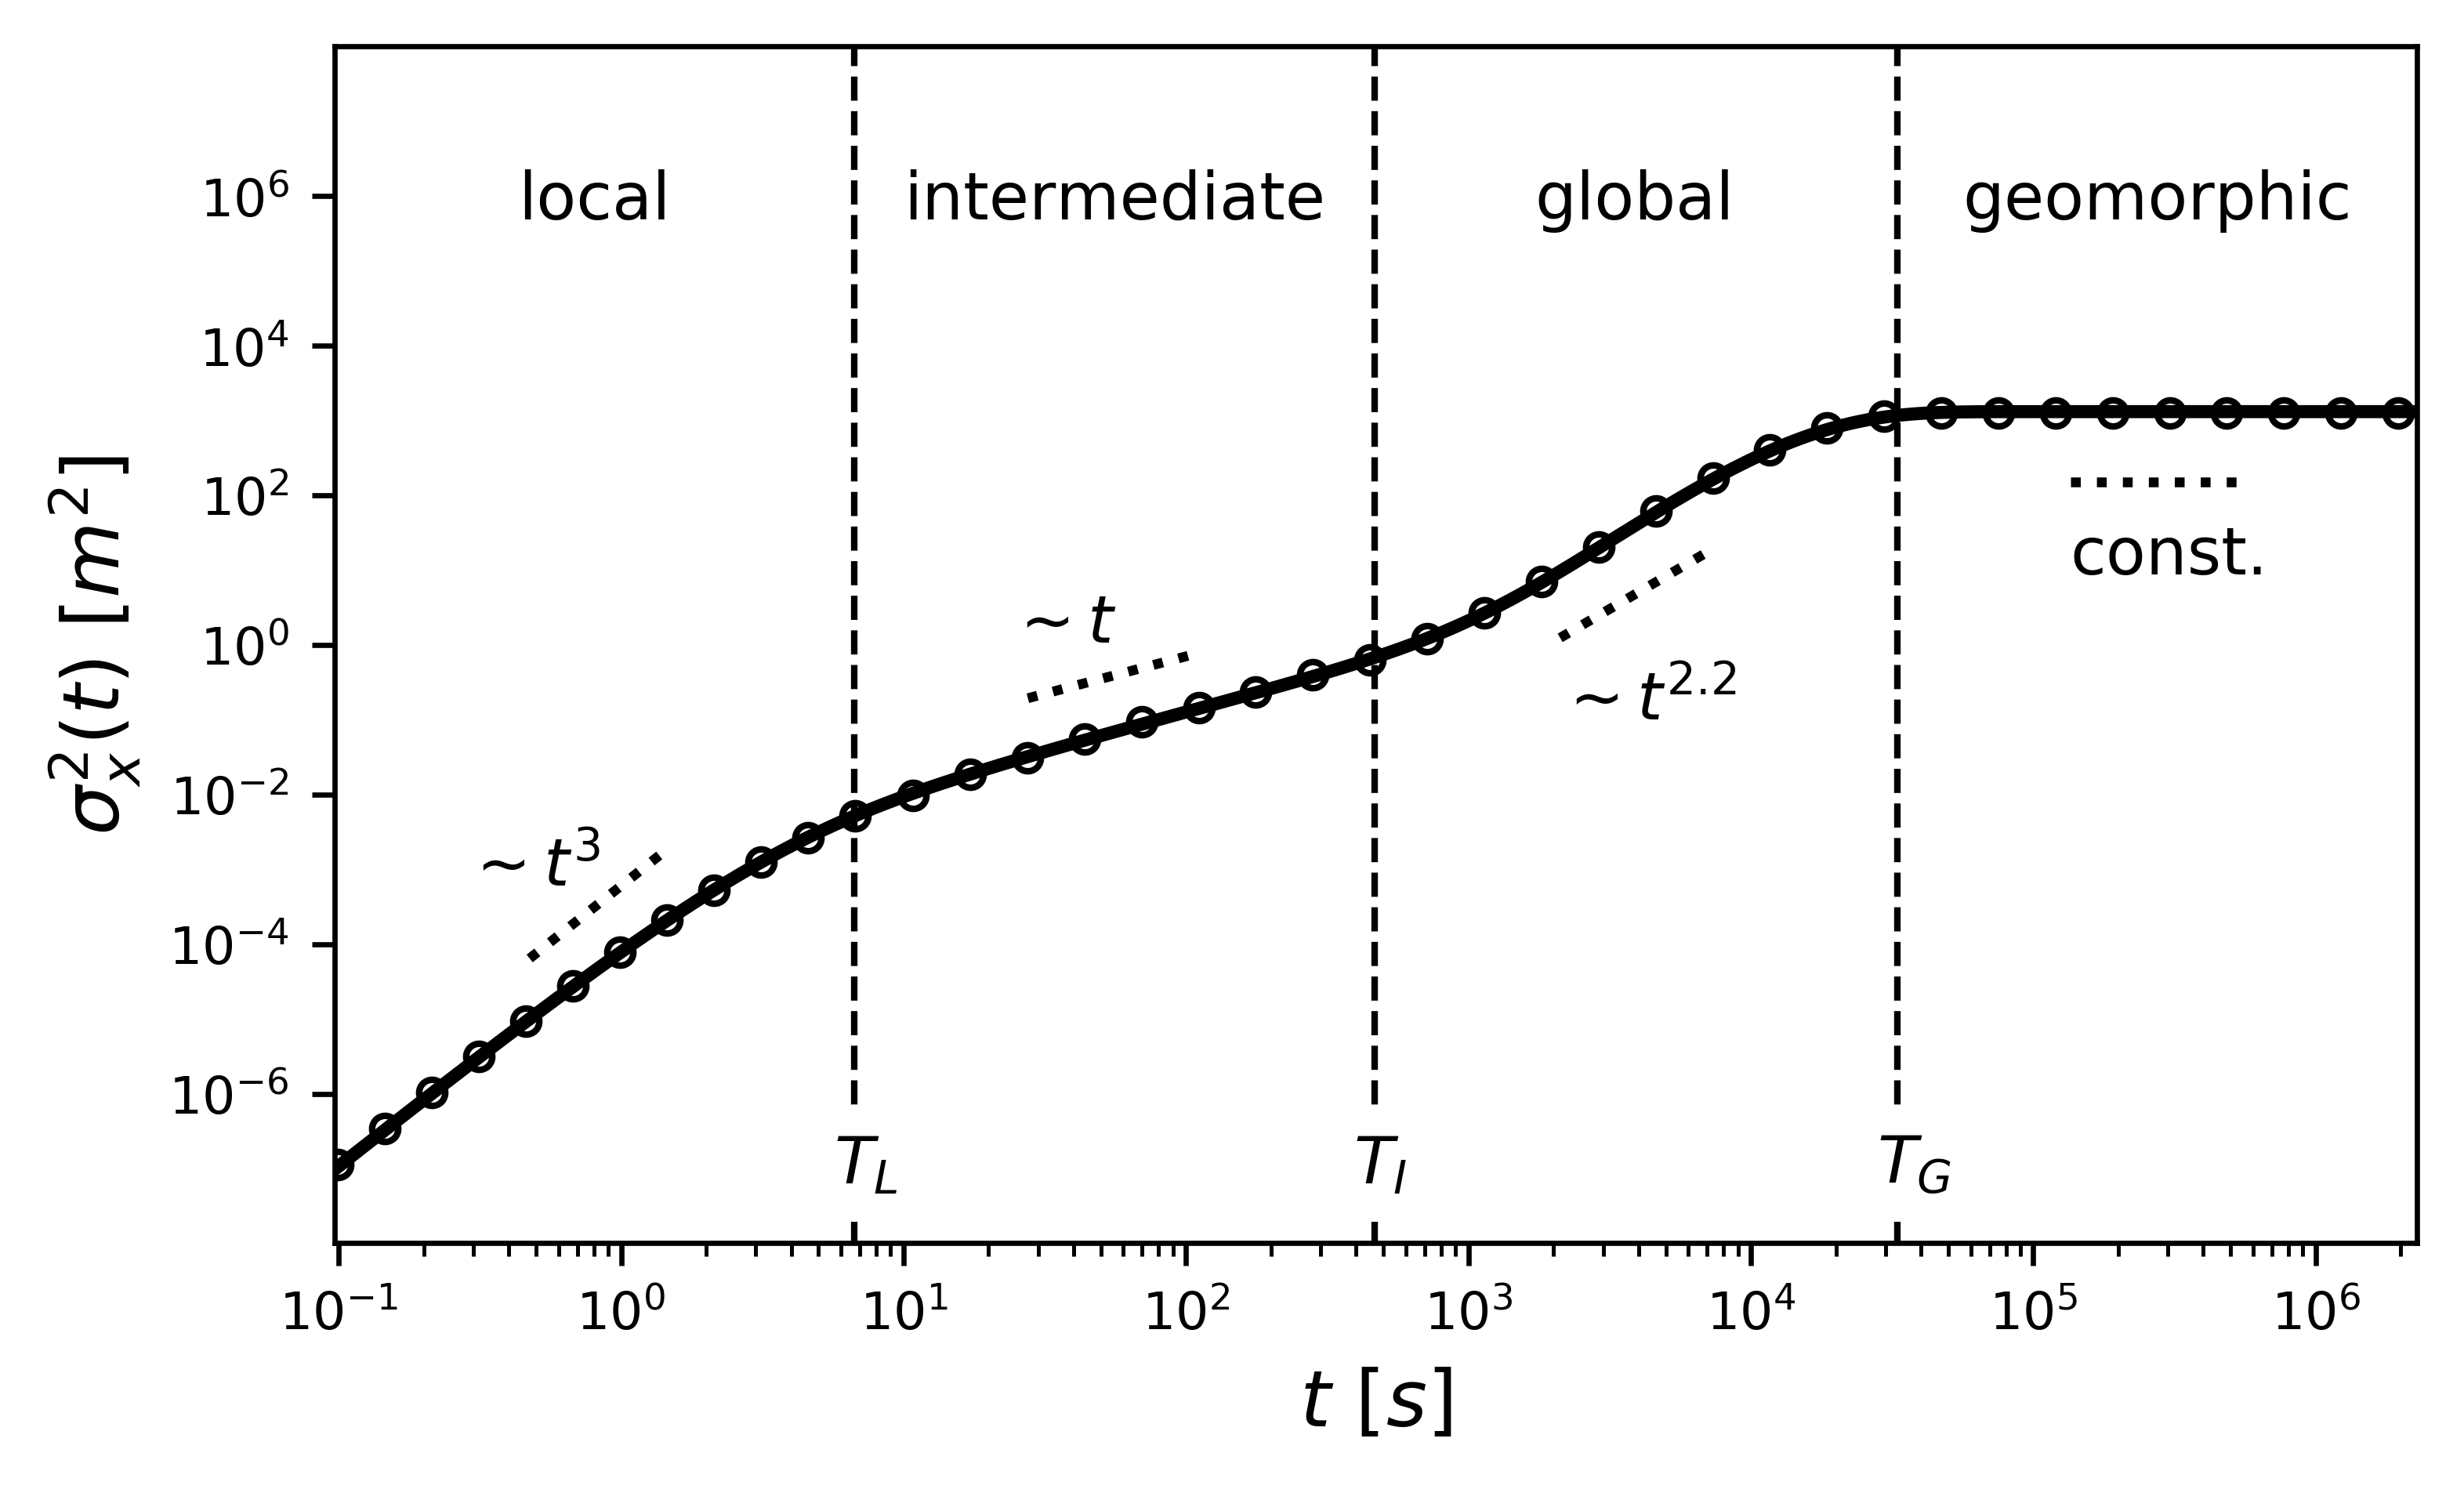
\includegraphics[width=\linewidth,keepaspectratio]{./figures/diffusion.png}
	\caption{The variance equation (\ref{eq:var}) is plotted for the parameters $1/k_2 = 1.5$s, $1/k_1 = 30.0$s, and $v=0.1$m/s. These values are comparable to laboratory flume experiments transporting small ($\sim 5$mm) gravels \citep[cf.,][]{Lajeunesse2010,Martin2012}. The timescale of burial is set to $1/\kappa = 7200.0$s (two hours), and the initial condition is rest ($\theta_1=1$). The solid line is equation (\ref{eq:var}) while the points are \change{directly}{numerically} simulated. When $k_2\gg k_1 \gg \kappa$\change{, as is the case}{as} in this plot, there are four distinct scaling ranges of $\sigma_x^2$: local, intermediate, global, and geomorphic. Within each range, a slope key is added to demonstrate the scaling $\sigma_x^2 \propto t^\gamma$. There are three crossovers between these ranges, denoted on the figure by vertical lines. Crossover times $T_L$, $T_I$, and $T_G$ are indicated at the bottom of the plot. They are given in equations (\ref{eq:TL}-\ref{eq:TG}) in terms of the model's input parameters. }
	\label{fig:var}
\end{figure}


% WORK HERE
\section{Discussion}
\label{sec:discussion}

The model we've presented \change{involves}{predicts three diffusion ranges for a group of bedload tracers transporting downstream as they gradually become buried, providing the first analytical description of Nikora's concept.} \change{in terms of}{The model requires} four parameters. These are the characteristic velocity $v$ of moving sediment and three \remove{key}timescales: $1/k_2$, $1/k_1$, and $1/\kappa$.
The timescales represent the mean durations of motion, rest, and rest before burial occurs.
As shown in figure \ref{fig:var}, scaling laws $\sigma_x^2 \propto t^\gamma$ approximately characterize the diffusion in each scaling range.
The exponents $\gamma$ in each range result from competition between different terms in equation (\ref{eq:var}).
Between these ranges, there are crossover regions where the scaling is not a simple power law.
Because these crossover regions are relatively narrow, we can approximately characterize them with crossover times $T_L$, $T_I$, and $T_G$.
These times partition the \remove{diffusion }ranges into $0< t < T_L$ (local), $T_L < t < T_I$ (intermediate), $T_I < t < T_G$ (global), and $T_G < t$ (geomorphic). 
Figure \ref{fig:var} depicts these crossover times as vertical lines.
To understand the scale dependence expressed by the bedload variance in equation (\ref{eq:var}), we need to determine the exponents $\gamma$ of each range and relate the crossover times $T_L$, $T_I$, and $T_G$ between diffusion ranges to the model parameters $v$, $k_1$, $k_2$, and $\kappa$.

% now we figure out what the exponents are 
We determine the diffusion exponents $\gamma$ in the local, intermediate, and global ranges using two limiting cases of equation (\ref{eq:var}): (1) $t\ll 1/\kappa$, and (2) $1/k_2 \rightarrow 0$ while $vk_2 = \text{constant}$.
Limit (1) corresponds to times so short a negligible amount of sediment burial has occurred, while limit (2) corresponds to times so long a motion interval appears as an instantaneous step having mean step length $l=vk_2$.
We evaluate these limits in \change{appendix \ref{sec:appendixC} and}{the supplementary information to} obtain the diffusion exponents.
Local range diffusion has exponent $2 \leq \gamma \leq 3$ depending on the initial conditions $\theta_1$ and $\theta_2$.
When the initial conditions are pure, meaning one of the $\theta_i$ is zero, the local exponent is $\gamma=3$.
When grains start in a mixture of motion and rest states, meaning neither $\theta_i$ is zero, the local exponent is $\gamma=2$.
Intermediate range diffusion always has exponent $\gamma=1$, agreeing with classic flume experiments \citep[e.g.,][]{Einstein1937,Yano1969a,Nakagawa1976}.
Finally, global range diffusion has exponent $1 < \gamma < 3$ depending on the ratio $k_1/\kappa$.
In the extreme case $k_1/\kappa \approx 0 $, we find normal diffusion $\sigma_x^2 \propto t$. 
However, in the opposite extreme $k_1/\kappa \rightarrow \infty$, we find  super-diffusion $\sigma_x^2 \propto t^3$.
For general ratios $\kappa/k_1$, the global exponent lies between these extremes.
For example, when $k_1/\kappa \approx 240$ as in figure \ref{fig:var}, the global range exponent is $\gamma \approx 2.2$. 
We surmise when the model parameters satisfy $k_2\gg k_1 \gg \kappa$, meaning all three diffusion ranges exist, the variance (\ref{eq:var}) implies local range super-diffusion with exponent depending on the $\theta_i$, intermediate range normal diffusion with no dependence on model parameters, and global range super-diffusion with exponent depending on the ratio $k_1/\kappa$.
Finally, the model supports a geomorphic range of no diffusion ($\gamma=0$) associated with the eventual and long term burial of all sediment grains.

Each of the three crossover times relates to a physical process affecting a population of grains.
Exchange between motion and rest states induces the local/intermediate crossover, the onset of sediment burial induces the intermediate/global crossover, and the completion of sediment burial induces the global/geomorphic crossover.
Each process admits two characteristic times, and we formulate the crossover times heuristically as geometric averages of these characteristic times:
\begin{alignat}{2}
&T_L &&= \sqrt{\frac{1}{k_1}\frac{1}{k_2}}, \label{eq:TL}\\
&T_I &&= \sqrt{\frac{1}{k_1}\frac{1}{\kappa}},\label{eq:TI}\\
&T_G &&= \sqrt{\frac{1}{\kappa}\frac{k_1+k_2}{\kappa k_1}} \label{eq:TG}.
\end{alignat}
Figure \ref{fig:var} depicts these relationships as dashed vertical lines.
The times $1/k_1$ and $1/k_2$ characterize exchanges between motion and rest, while $1/k_1$ and $1/\kappa$ characterize the onset of burial originating from grains buried in their first resting sojourns.
Equations (\ref{eq:TL}) and (\ref{eq:TI}) mix these paired times.
The completion of sediment burial and its characteristic timescales originate from the last grains to bury.
In one extreme, all grains rest on the surface, meaning the last grains bury around $1/\kappa$; while in another, a fraction of grains remains in motion for a long time evading burial.
By analogy to the mobile-immobile model of \citet{Ancey2006}, we reason that a fraction $k_1/(k_1+k_2)$ of the free population will be in motion and evading burial at long timescales, and for this fraction we propose an effective trapping rate $\kappa k_1/(k_1+k_2)$.
Equation (\ref{eq:TG}) mixes the reciprocal of this effective rate with $1/\kappa$.
We tested formulas (\ref{eq:TL}-\ref{eq:TG}) for many parameter choices and conclude they adequately represent the crossover locations between diffusion regimes provided the parameters satisfy $k_2\gg k_1 \gg \kappa$ and grains start from rest ($\theta_1=1$).
However, starting grains from motion ($\theta_2=1$) widens the crossover region between local and intermediate ranges, meaning equation (\ref{eq:TL}) loses representative power; while setting relatively very large values of $k_2$ widens the crossover region between global and geomorphic ranges, meaning equation (\ref{eq:TG}) loses representative power.
Ultimately, we emphasize the representation of finite width crossover regions by crossover times is an idealization, so we propose equations (\ref{eq:TL}-\ref{eq:TG}) as heuristics. 
These relations provide useful divisions between the bedload diffusion scaling ranges.

Our \change{four}{three} range bedload diffusion model reduces to earlier works through the two simplified limits previously leveraged to extract the scaling exponents $\gamma$ and \change{explored in appendix \ref{sec:appendixC}.}{described in the supplementary information}.
Limit (1) implies the model developed by \citet{Lisle1998} to describe soil transport within a sheet flow, while limit (2) implies the model developed by \citet{Wu2019} to describe bedload transport with burial.
Either of these cases further simplifies to the classic results of \citet{Einstein1937} and his early followers \citep[e.g.,][]{Hubbell1964, Nakagawa1976, Yano1969} that predict a single range of normal diffusion.
\citet{Lisle1998} generalized the Einstein model to include a finite velocity and duration of motion in place of instantaneous steps, and they derived two ranges of diffusion -- super-diffusive and normal.
\citet{Wu2019} developed an active layer formulation of bedload transport where grains are transferred from the active layer (surface) to the substrate layer (burial) at a constant rate.
They simplified the problem by interpreting motions as instantaneous steps, and they derived two ranges of diffusion -- normal and super-diffusive.
Our model ultimately extends these two works and re-frames them in the formalism of CTRWs \citep[e.g.,][]{Weiss1994} that was implicitly applied by \citet{Einstein1937}.

We offer several implications of our model for bedload diffusion studies in gravel bed streams.
First, our model confines the valid range of scale independent models such as the advection-diffusion equation \citep[e.g.,][]{Bradley2010} and the Einstein model \citep[e.g.,][]{Martin2012} for practical applications such as contaminant transport \citep[e.g][]{Malmon2005,Macklin2006} and aquatic habitat restoration \citep[e.g.,][]{Gaeuman2017}.
We can conclude when the observation timescale satisfies $T_L<t<T_I$, with $T_L$ and $T_I$ given by equations (\ref{eq:TL}) and (\ref{eq:TI}), we expect normal bedload diffusion $\sigma_x^2 = D_d t$.
For example, if grains move for a mean duration $0.5$s, they rest for a mean duration $1$hr, and burial takes, on average $30$hr for resting grains, a normal diffusion model such as \citet{Einstein1937} would be applicable for observation times between $T_L \approx 1.2$min and $T_I \approx 5.5$hr.
Second, the model links bedload transport understanding across scales. 
In practice, we might measure sediment diffusion within a channel on one timescale with intent to apply our knowledge at smaller or larger timescales; usually, experimental limitations constrain the measurement timescale.
For example, we could determine $k_1$ and $k_2$ by measuring the virtual velocity and diffusivity of sediment tracers in the intermediate range \citep[e.g.,][]{Einstein1937,Yano1969a,Nakagawa1976}.
With an estimate of the trapping rate $\kappa$, equation (\ref{eq:var}) provides diffusion characteristics of the global range $T_I<t<T_G$ which is more difficult to study experimentally.

To describe the scale dependence of bedload diffusion, we extended the original Einstein model by building up ideas from condensed matter physics.
Along the way, we incorporated two simplifying assumptions that deserve further research attention. 
First, we treated sediment burial as a quasi permanent condition; and second, we implicitly assumed burial is the only process trapping grains in river channels.
In actuality, burial is a temporary condition linked to scour and fill of the sedimentary bed \citep{Hassan1994,Voepel2013,Martin2014,Wu2019a}, and field experiments show other processes trapping sediment.
For example, grains can become stranded on bars \citep{Ferguson2002,Bradley2017} and embedded in stabilizing structures such as steps or clusters \citep[e.g.][]{Church1998,Hassan2008}.
In principle, the multi state CTRW framework we developed here can describe bedload diffusion with multiple trapping processes by simply adding more states, and it can handle impermanent sojourns in these states by specifying propagators for them.
Unfortunately, we currently lack the experimental knowledge to specify these propagators, since trapping rates and durations are poorly understood in association with particular processes.
For example, recent experiments have attributed resting times to any immobile sediment, and this is known to imply heavy-tailed sediment resting time distributions \citep[e.g.,][]{Olinde2015,Bradley2017}.
However, \change{very few studies have}{only one study has} resolved immobile times of sediment while identifying their underlying mechanism \citep{Martin2014}.
We propose experiments to determine the rates and durations of specific bedload trapping processes are important topics for further study.
A first step might be to measure the burial rate $\kappa$ we applied in this paper; in principle, this could be discerned by timing the period required for tagged surface grains to become buried in flume experiments.
Once better understanding of the rates and durations of sediment trapping processes is in place, generalizations built from the framework we've presented in this paper should better predict bedload diffusion on the global and geomorphic scales.


\section{Conclusion}
\label{sec:conclusion}
We developed a random walk model \remove{with alternating mobile and immobile states and a possibility of trapping from the immobile state, and we used it }to describe \change{sediment transporting through a river channel as it gradually becomes buried}{a group of sediment grains transporting through a river channel as it gradually becomes buried}.
To our knowledge, this is the first analytical description of bedload diffusion \change{across}{capturing} the local, intermediate, and global timescales introduced by \citet{Nikora2001a}.
Pushing the ideas of Nikora somewhat further, we proposed a geomorphic range to describe diffusion characteristics at timescales larger than the global range.
At base level, our model demonstrates the required components for three bedload diffusion ranges: (1) the duration of sediment motions, (2) mobile-immobile switching, and (3) a sediment trapping process.
A next step is to incorporate the bed scour process that re-exposes buried sediment to better understand the global and geomorphic ranges.
Ultimately, we emphasize the multi state random walk formalism used in this paper implicitly underlies most existing bedload diffusion models, and we believe it will readily accommodate efforts to include more physical processes into Einstein's research paradigm.

\appendix


\acknowledgments
J. Pierce acknowledges a helpful exchange with Eduardo Daly during the early stages of this work. He would like to thank Melinda Saunders and Leonardo Golubovic for their careful guidance in mathematics through the years. M. Hassan is supported by an NSERC Discovery grant. The Python simulation code is available at \sloppy
\url{https://github.com/jkpierce/rw-diffu}.

\bibliography{biblio.bib}
\end{document}
